\section{色覚異常とカラーユニバーサルデザイン(CUD)について}
本章では,色覚異常とCUDについて説明する.

\subsection{色覚異常について}
人間の目には,赤,緑,青の3種類をそれぞれ感じる機能を持つ錐体があり,その錐体によって色を識別している.
この錐体の一部が十分に機能しないために,通常とは色の見え方が異なる色覚となる場合がある.
このような色覚を持つ色覚異常者は,日本人の場合,男性で5%,女性で0.2%存在する.

色覚異常者は,主にどの色を感じづらい色覚かによって区別される.
主に赤を感じづらい色覚であるP型色覚は,全体の約25%を占める.
主に緑を感じづらい色覚であるD型色覚は,全体の約75%を占める.
主に青を感じづらい色覚であるT型色覚は,全体の約0.02%を占める.

\subsection{色覚異常の見え方とCUDについて}
図\ref{fig:pcolor_mae}は,同じグラフに対しての色覚による見え方の違いを表している.
左は通常の色覚での見え方,右はP型色覚での見え方を表している.
線1は緑色,線2は赤色であり,通常の色覚では区別がつきやすい.
しかし,P型色覚ではどちらも茶色に近い色に見えるため区別がつきづらい.
このように,通常の色覚者には伝わりやすい情報であっても,色覚異常者には伝わりづらくなっている場合がある.

\begin{figure}[h]
\begin{center}
 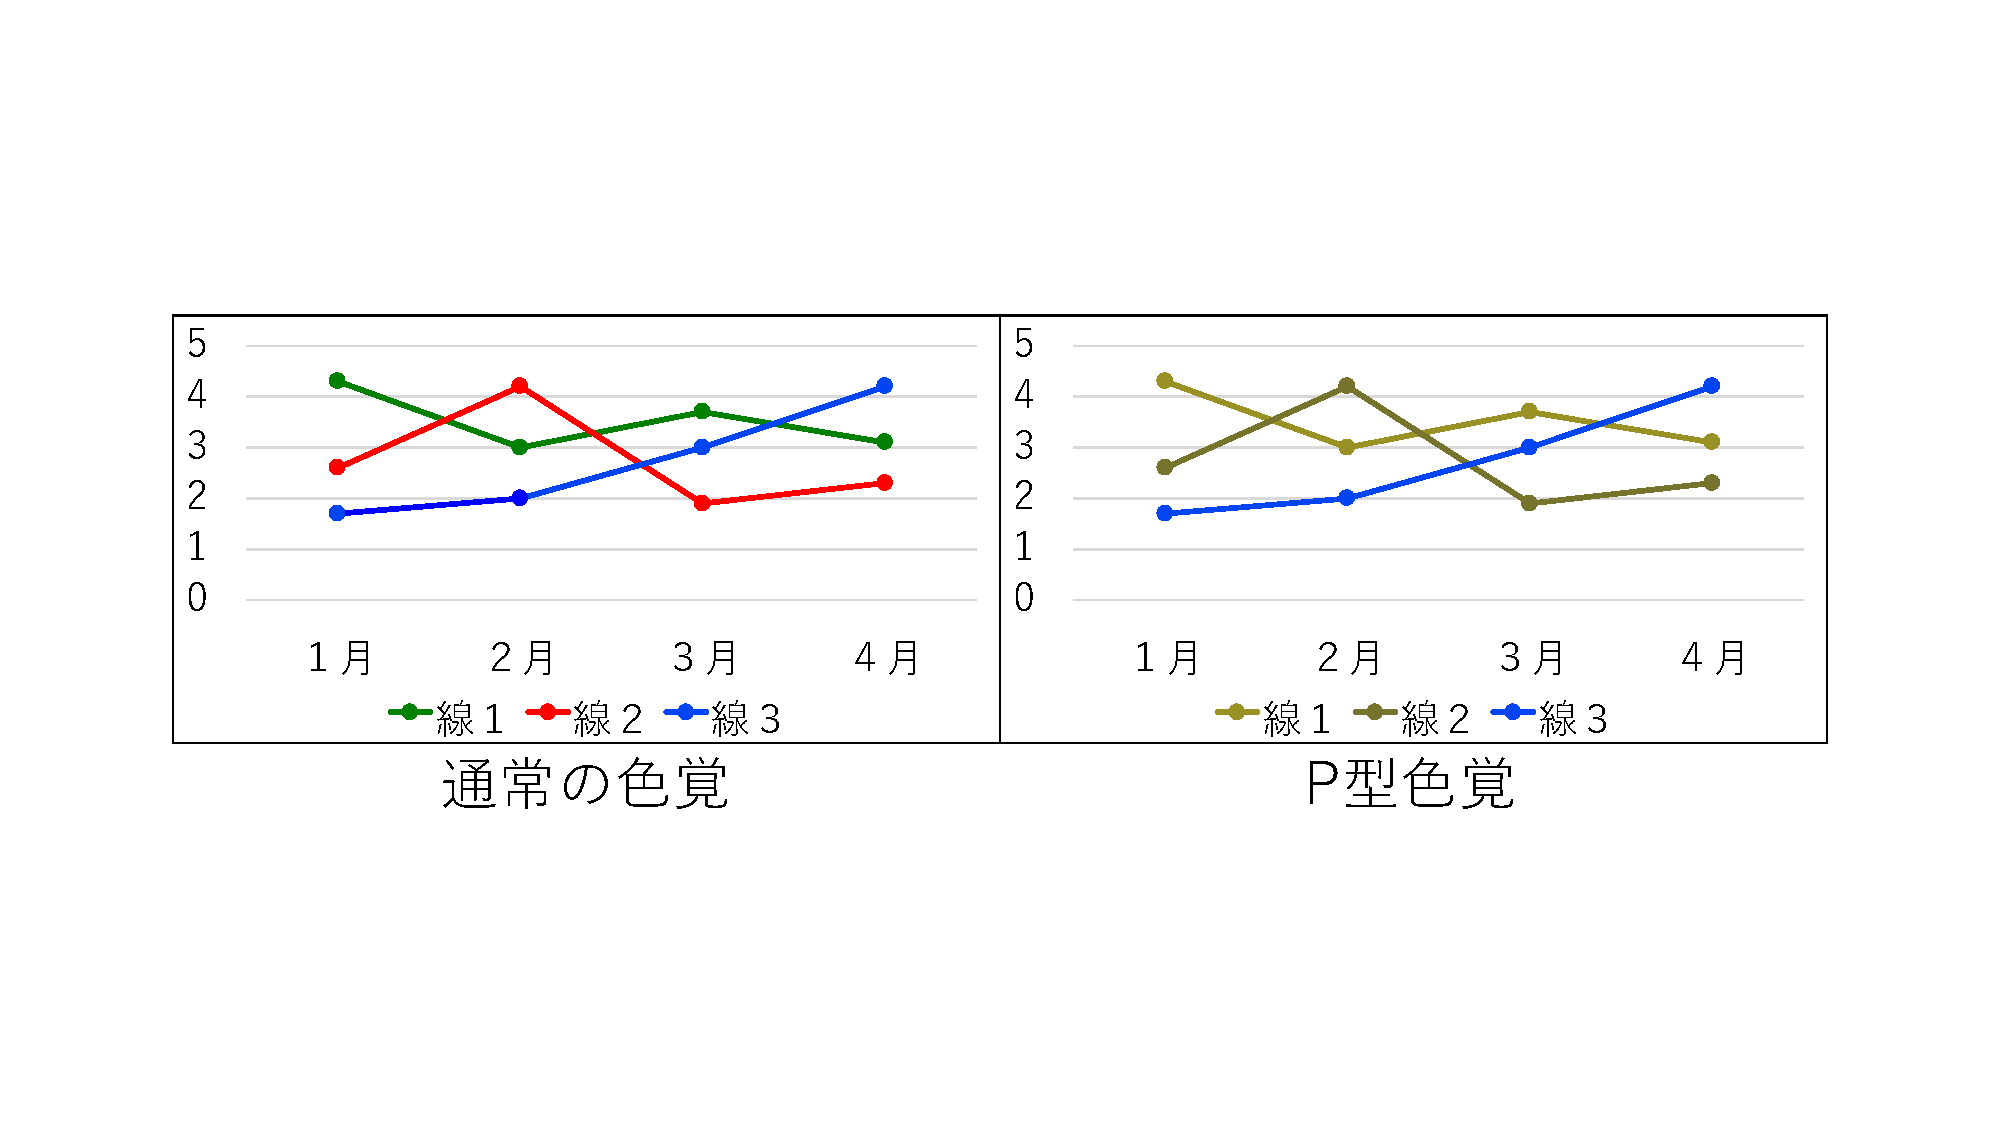
\includegraphics[clip,width=160mm,height=48mm]{images/pcolor_mae.pdf}
\end{center}
 \caption{P型色覚者の見え方}
 \label{fig:pcolor_mae}
\end{figure}

\clearpage

色覚の多様性に配慮し,より多くの人に伝わりやすい配色やデザインとして,CUDがある.
図\ref{fig:pcolor_ato}は,図\ref{fig:pcolor_ato}のグラフをCUDに配慮し,改善した例である.
図\ref{fig:pcolor_mae}と同様,左は通常の色覚での見え方,右はP型色覚での見え方を表している.
改善後のグラフでは,線2を橙色にし,点線にすることで区別がつきやすくした.
このように,色覚異常者にも正確に伝えるためには,CUDに配慮する必要がある.

\begin{figure}[h]
\begin{center}
 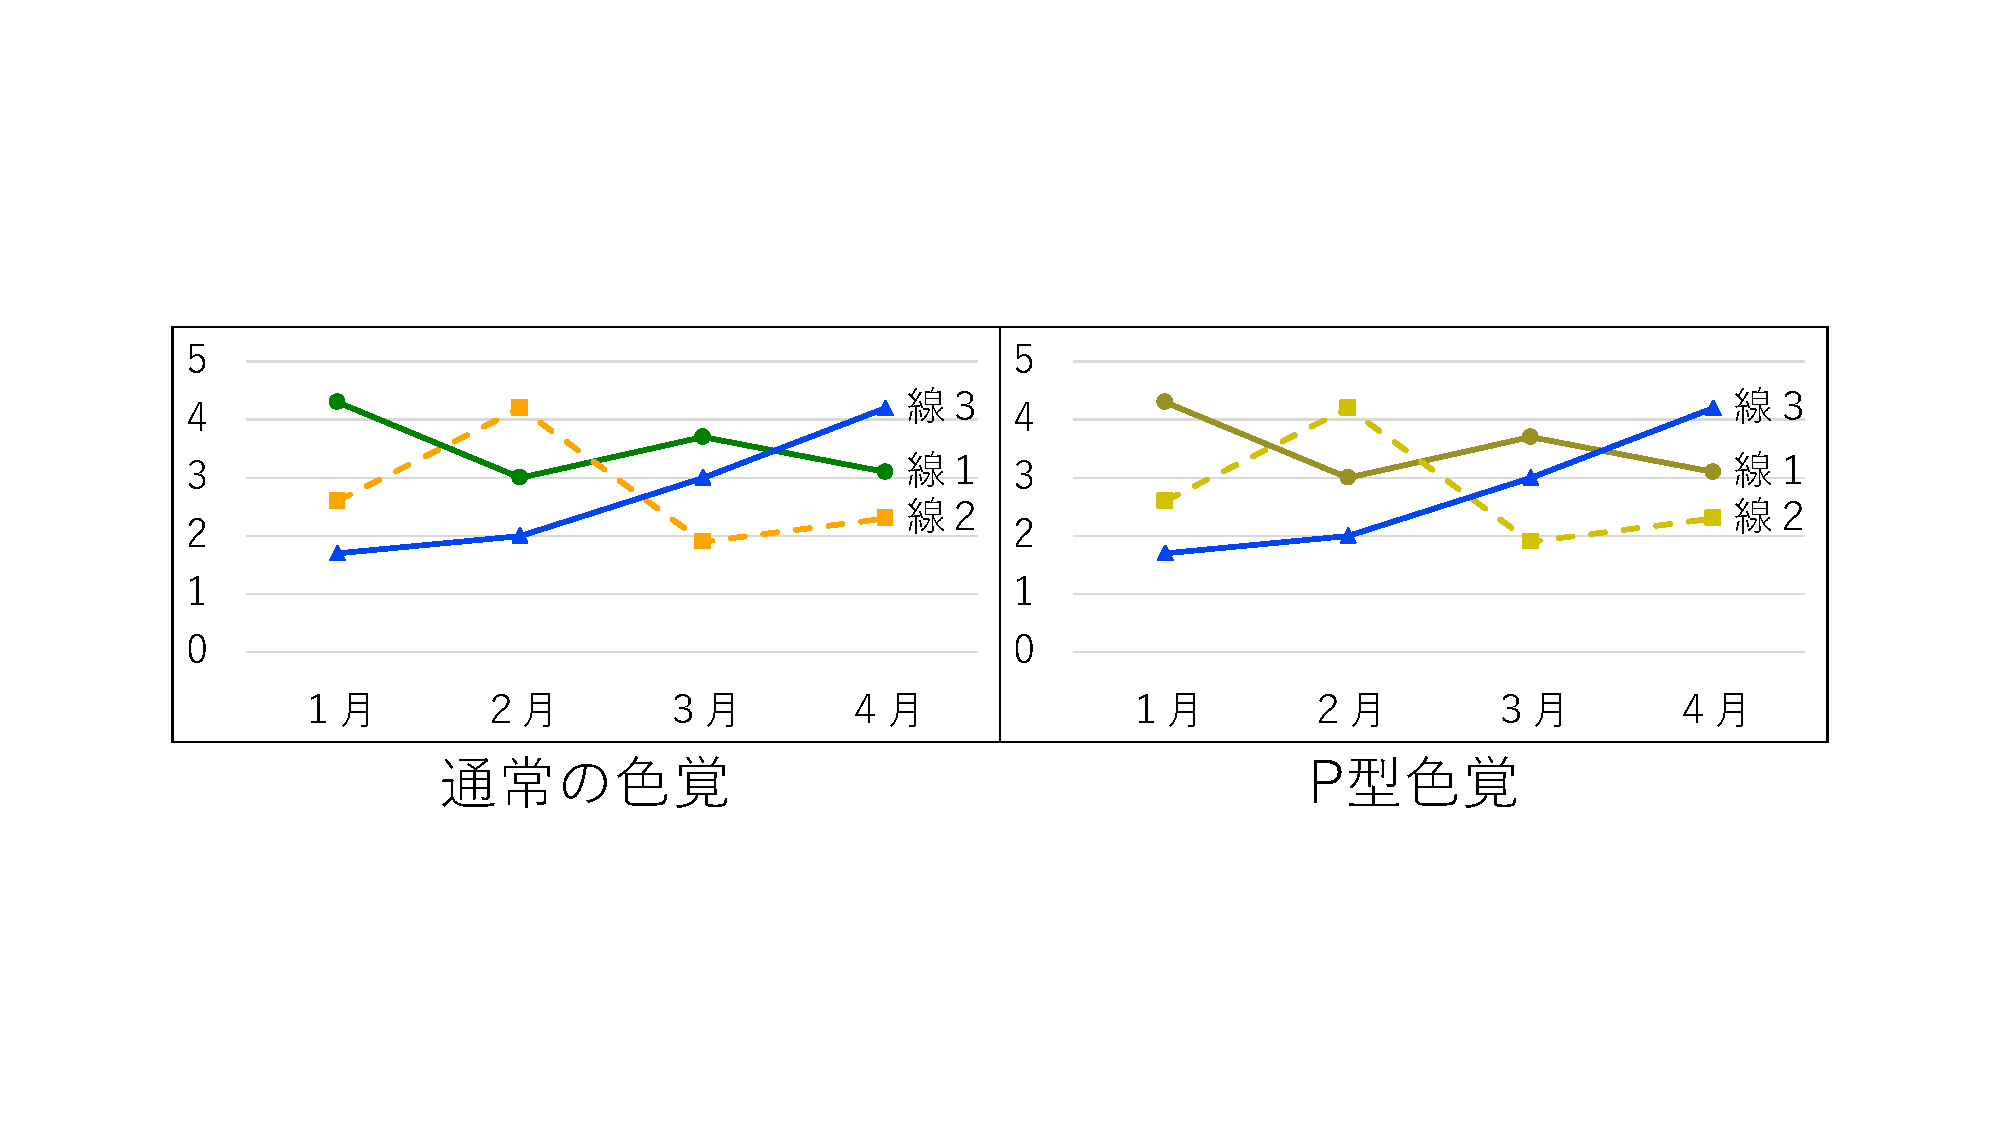
\includegraphics[clip,width=159mm,height=47mm]{images/pcolor_ato.pdf}
\end{center}
 \caption{改善後のグラフの見え方}
 \label{fig:pcolor_ato}
\end{figure}

\subsection{CUDの普及に向けた活動}
CUDの普及に向けた活動として,東京都は「カラーユニバーサルデザインガイドライン」を作成している\cite{tokyo}.
また,大阪府は「色覚障がいのある人に配慮した色使いのガイドライン」を作成している\cite{osaka}.
これらのように,一部の自治体がCUDの認知度を高めることを目的とし,CUDのガイドラインを作成している.

また,一部の大学,専門学校や会社では,講義や研修等を通してCUDに関する講習を行っている.



